\documentclass[11pt,a4paper]{article}

% ------------------------------------------------------------------
% Packages
% ------------------------------------------------------------------
\usepackage[a4paper,margin=2cm]{geometry}
\usepackage[T1]{fontenc}
\usepackage{lmodern}
\usepackage{microtype}
\usepackage{amsmath,amssymb}
\usepackage{graphicx}
\usepackage{booktabs,tabularx,multirow,array}
\usepackage{xcolor}
\usepackage{enumitem}
\usepackage{caption}
\usepackage{subcaption}
\usepackage{float}
\usepackage{tikz}
\usetikzlibrary{positioning,arrows.meta,fit,backgrounds,calc,shapes.geometric}
\usepackage{pgfplots}
\pgfplotsset{compat=1.17}
\usepgfplotslibrary{fillbetween}
\usepackage{titlesec}
\usepackage{fancyhdr}
\usepackage[hidelinks]{hyperref}

\setlist{itemsep=1pt,topsep=3pt,parsep=0pt,leftmargin=1.4em}
\captionsetup{font=small,labelfont=bf,margin=0.5em}
\titleformat{\section}{\large\bfseries\color{ink}}{\thesection}{0.6em}{}
\titleformat{\subsection}{\normalsize\bfseries\color{ink}}{\thesubsection}{0.6em}{}
\titlespacing*{\section}{0pt}{10pt}{4pt}
\titlespacing*{\subsection}{0pt}{7pt}{2pt}
\setlength{\parskip}{3pt}
\setlength{\parindent}{0pt}

% ------------------------------------------------------------------
% Colours
% ------------------------------------------------------------------
\definecolor{ink}{HTML}{1F2937}
\definecolor{vid}{HTML}{2563EB}     % video / online path
\definecolor{sen}{HTML}{059669}     % sensor / offline path
\definecolor{fus}{HTML}{7C3AED}     % fusion
\definecolor{outc}{HTML}{DC2626}    % output
\definecolor{val}{HTML}{6B7280}     % validation
\definecolor{cStance}{HTML}{FEF3C7}
\definecolor{cBack}{HTML}{DBEAFE}
\definecolor{cDown}{HTML}{FFEDD5}
\definecolor{cImp}{HTML}{FEE2E2}
\definecolor{cFT}{HTML}{EDE9FE}
\definecolor{fOK}{HTML}{16A34A}
\definecolor{fOCC}{HTML}{F59E0B}
\definecolor{fCAM}{HTML}{8B5CF6}
\definecolor{fBLUR}{HTML}{DC2626}

\newcommand{\kmh}{\,km/h}
\newcommand{\pxs}{\,px/s}

\pagestyle{fancy}
\fancyhf{}
\renewcommand{\headrulewidth}{0.3pt}
\fancyhead[L]{\small\color{val} str8bat AI Engineer Take-Home}
\fancyhead[R]{\small\color{val} Bat speed from broadcast video}
\fancyfoot[C]{\small\thepage}

% ------------------------------------------------------------------
\begin{document}
% ------------------------------------------------------------------

\begin{center}
{\LARGE\bfseries\color{ink} Bat Speed Across the Swing from Broadcast Video}\\[4pt]
{\large Using an unpaired library of sensor-recorded shots}\\[6pt]
{\small str8bat AI Engineer Technical Take-Home \quad$\cdot$\quad Part 1: System Design \quad$\cdot$\quad Part 2: Prototype on real footage}\\[2pt]
{\small Devansh Mittal}
\end{center}

\vspace{-2pt}
\noindent\colorbox{gray!8}{\parbox{\dimexpr\linewidth-2\fboxsep}{\small
\textbf{Summary.} Broadcast video tells us \emph{where} the batter's hands and bat are, roughly and in 2D, about 25 times a second.
The sensor library tells us \emph{what real swings look like}: dense, 3D-consistent, 100-sample bat-speed curves for millions of shots.
Neither is enough alone, and they are not paired. My design bridges them through \textbf{simulation}: sensor swings are rendered into synthetic
broadcast-style 2D observations, which gives unlimited paired training data, and the real clip is then explained by the most likely sensor-like swing
that reprojects onto what the camera saw. Metric scale comes from regulation pitch geometry, not from the prior.
The output is a 100-sample bat-speed curve $v(\tau)$, an impact speed, and an uncertainty band.
Part~2 runs the observation front-end on a real 72-frame clip: wrist tracking, a velocity profile in px/s and km/h,
and a frame-by-frame account of where tracking broke (74\% of shot frames were flagged) and why.}}

% ==================================================================
\section{Part 1: System design}
% ==================================================================

\subsection{What the system must produce, and what makes it hard}
For one shot in a broadcast clip, the target is the same quantity the sensor records: bat speed at each of $\sim$100 samples across the swing,
$v(\tau)$ for $\tau=1,\dots,100$, plus impact speed $v(\tau_{\text{imp}})$. Four properties of broadcast video make naive pixel differentiation fail:
\begin{itemize}
  \item \textbf{No calibration, moving camera.} The operator pans and zooms, and the director cuts. Pixel motion mixes batter and camera.
  \item \textbf{Depth loss.} The main camera looks down the pitch, so a straight drive moves largely \emph{along} the line of sight and looks slow in 2D.
  \item \textbf{Too few frames.} A downswing lasts about 150--200\,ms: 4--5 frames at 25--30\,fps, and some of those may be pulldown duplicates (Part~2 found one exactly at impact).
  \item \textbf{The bat is the hardest thing to see.} It is thin, fast and blurred at peak speed, and often hidden by the body in stance and follow-through.
\end{itemize}

\subsection{Key assumptions (made explicit)}
\begin{enumerate}[label=\textbf{A\arabic*}]
  \item \textbf{Sensor content.} Each record has per-sample bat speed and impact speed. I assume it \emph{also} has bat orientation or angular rate (typical for a bat-mounted IMU). If it only has speed, the prior is learned on speed curves alone and the swing plane comes from video (Section~\ref{sec:risks}).
  \item \textbf{Known sample timing.} The 100 samples have a consistent definition: either a fixed rate, or a phase-normalised window with an identifiable impact index. Without this, video time cannot be mapped onto $\tau$.
  \item \textbf{Standard geometry.} Stumps are 0.711\,m tall and the crease markings are regulation, so they are a free calibration target. Bat length is about 0.85\,m, and the sweet spot is 0.55--0.65\,m from the top hand.
  \item \textbf{Shape transfers, scale may not.} The sensor library (probably mostly amateur and club players) covers the \emph{shape} of elite swings, but not necessarily their \emph{magnitude}.
  \item \textbf{Usable footage.} The batter is in shot from stance to early follow-through on the main camera, at 25--50\,fps, at least 720p.
\end{enumerate}

\subsection{Architecture}
Figure~\ref{fig:arch} shows the end-to-end system. The blue path runs per clip. The green path runs offline, once, on the sensor library. They meet in the fusion stage (purple).

\begin{figure}[H]
\centering
\resizebox{\linewidth}{!}{%
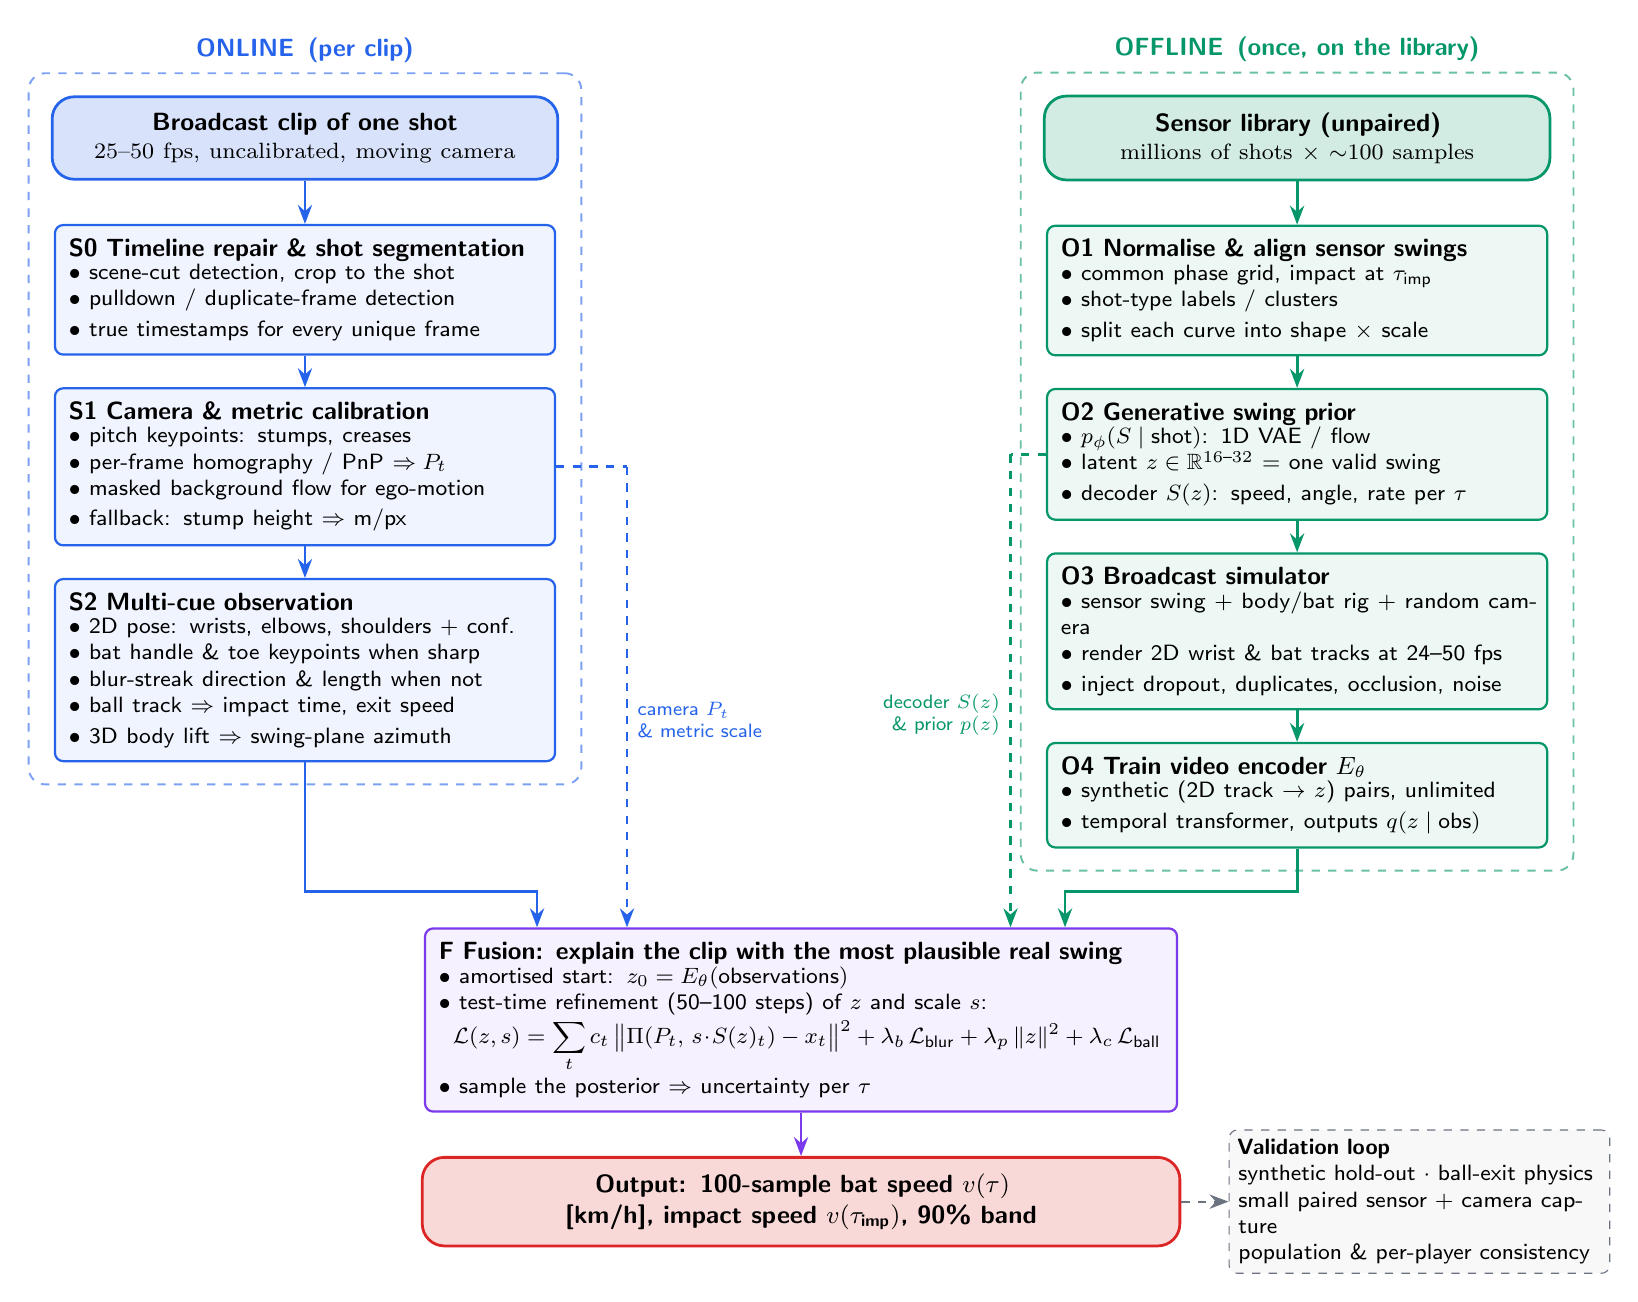
\begin{tikzpicture}[
  font=\sffamily\small,
  >={Stealth[length=2.4mm]},
  box/.style={draw=#1, fill=#1!7, rounded corners=3pt, line width=0.8pt,
              align=left, inner sep=5pt, text width=6.0cm},
  hdr/.style={font=\sffamily\bfseries\small, text=#1},
  io/.style={draw=#1, fill=#1!18, rounded corners=8pt, line width=1pt,
             align=center, inner sep=6pt, text width=6.0cm, font=\sffamily\bfseries\small},
  arr/.style={->, line width=1pt, draw=#1},
  lane/.style={draw=#1!60, dashed, rounded corners=6pt, line width=0.7pt, inner sep=8pt}
]
% ---------------- Inputs
\node[io=vid] (video) at (0,0) {Broadcast clip of one shot\\[-1pt]{\normalfont\footnotesize 25--50 fps, uncalibrated, moving camera}};
\node[io=sen] (lib) at (12.6,0) {Sensor library (unpaired)\\[-1pt]{\normalfont\footnotesize millions of shots $\times$ $\sim$100 samples}};

% ---------------- Online lane
\node[box=vid, below=0.55cm of video] (s0) {%
  \textbf{S0  Timeline repair \& shot segmentation}\\[-1pt]
  \footnotesize $\bullet$ scene-cut detection, crop to the shot\\
  $\bullet$ pulldown / duplicate-frame detection\\
  $\bullet$ true timestamps for every unique frame};
\node[box=vid, below=0.4cm of s0] (s1) {%
  \textbf{S1  Camera \& metric calibration}\\[-1pt]
  \footnotesize $\bullet$ pitch keypoints: stumps, creases\\
  $\bullet$ per-frame homography / PnP $\Rightarrow P_t$\\
  $\bullet$ masked background flow for ego-motion\\
  $\bullet$ fallback: stump height $\Rightarrow$ m/px};
\node[box=vid, below=0.4cm of s1] (s2) {%
  \textbf{S2  Multi-cue observation}\\[-1pt]
  \footnotesize $\bullet$ 2D pose: wrists, elbows, shoulders + conf.\\
  $\bullet$ bat handle \& toe keypoints when sharp\\
  $\bullet$ blur-streak direction \& length when not\\
  $\bullet$ ball track $\Rightarrow$ impact time, exit speed\\
  $\bullet$ 3D body lift $\Rightarrow$ swing-plane azimuth};

% ---------------- Offline lane
\node[box=sen, below=0.55cm of lib] (o1) {%
  \textbf{O1  Normalise \& align sensor swings}\\[-1pt]
  \footnotesize $\bullet$ common phase grid, impact at $\tau_{\text{imp}}$\\
  $\bullet$ shot-type labels / clusters\\
  $\bullet$ split each curve into shape $\times$ scale};
\node[box=sen, below=0.4cm of o1] (o2) {%
  \textbf{O2  Generative swing prior}\\[-1pt]
  \footnotesize $\bullet$ $p_\phi(S \mid \text{shot})$: 1D VAE / flow\\
  $\bullet$ latent $z\in\mathbb{R}^{16\text{--}32}$ = one valid swing\\
  $\bullet$ decoder $S(z)$: speed, angle, rate per $\tau$};
\node[box=sen, below=0.4cm of o2] (o3) {%
  \textbf{O3  Broadcast simulator}\\[-1pt]
  \footnotesize $\bullet$ sensor swing + body/bat rig + random camera\\
  $\bullet$ render 2D wrist \& bat tracks at 24--50 fps\\
  $\bullet$ inject dropout, duplicates, occlusion, noise};
\node[box=sen, below=0.4cm of o3] (o4) {%
  \textbf{O4  Train video encoder $E_\theta$}\\[-1pt]
  \footnotesize $\bullet$ synthetic (2D track $\to$ $z$) pairs, unlimited\\
  $\bullet$ temporal transformer, outputs $q(z\mid\text{obs})$};

% ---------------- Fusion
\path (o4.south) ++(0,-1.0) coordinate (fy);
\coordinate (mid) at ($(s2.south)!0.5!(o4.south)$);
\node[box=fus, text width=9.2cm, anchor=north] (f) at (mid |- fy) {%
  \textbf{F  Fusion: explain the clip with the most plausible real swing}\\[-1pt]
  \footnotesize $\bullet$ amortised start: $z_0 = E_\theta(\text{observations})$\\
  $\bullet$ test-time refinement (50--100 steps) of $z$ and scale $s$:\\[1pt]
  \hspace*{0.6em}$\displaystyle \mathcal{L}(z,s)=\sum_t c_t\,\big\|\Pi(P_t,\,s\!\cdot\!S(z)_t)-x_t\big\|^2
   + \lambda_b\,\mathcal{L}_{\text{blur}} + \lambda_p\,\|z\|^2 + \lambda_c\,\mathcal{L}_{\text{ball}}$\\[1pt]
  $\bullet$ sample the posterior $\Rightarrow$ uncertainty per $\tau$};

\node[io=outc, text width=9.2cm, below=0.55cm of f] (out) {%
  Output: 100-sample bat speed $v(\tau)$ [km/h], impact speed $v(\tau_{\text{imp}})$, 90\% band};

% ---------------- Arrows
\draw[arr=vid] (video) -- (s0);
\draw[arr=vid] (s0) -- (s1);
\draw[arr=vid] (s1) -- (s2);
\draw[arr=sen] (lib) -- (o1);
\draw[arr=sen] (o1) -- (o2);
\draw[arr=sen] (o2) -- (o3);
\draw[arr=sen] (o3) -- (o4);
\draw[arr=vid] (s2.south) |- ($(f.north west)!0.15!(f.north east)+(0,0.45)$) -- ($(f.north west)!0.15!(f.north east)$);
\draw[arr=sen] (o4.south) |- ($(f.north west)!0.85!(f.north east)+(0,0.45)$) -- ($(f.north west)!0.85!(f.north east)$);
\draw[arr=fus] (f) -- (out);
% prior feeds fusion directly (decoder + prior term)
\draw[sen, dashed, line width=1pt] (o2.west) -- ($(o2.west)+(-0.45,0)$) coordinate (pa);
\draw[arr=sen, dashed] (pa) -- (pa |- f.north) node[pos=0.55, left, font=\sffamily\scriptsize, text=sen, align=right]{decoder $S(z)$\\ \& prior $p(z)$};
% calibration feeds fusion
\draw[vid, dashed, line width=1pt] (s1.east) -- ($(s1.east)+(0.9,0)$) coordinate (ca);
\draw[arr=vid, dashed] (ca) -- (ca |- f.north) node[pos=0.55, right, font=\sffamily\scriptsize, text=vid, align=left]{camera $P_t$\\ \& metric scale};

% ---------------- Lanes
\begin{scope}[on background layer]
\node[lane=vid, fit=(video)(s0)(s1)(s2), label={[hdr=vid]above:ONLINE \,(per clip)}] {};
\node[lane=sen, fit=(lib)(o1)(o2)(o3)(o4), label={[hdr=sen]above:OFFLINE \,(once, on the library)}] {};
\end{scope}

% ---------------- Validation
\node[draw=val, dashed, rounded corners=3pt, fill=val!5, align=left, text width=4.6cm,
      font=\sffamily\footnotesize, right=0.6cm of out, anchor=west] (v) {%
  \textbf{Validation loop}\\
  synthetic hold-out $\cdot$ ball-exit physics\\
  small paired sensor + camera capture\\
  population \& per-player consistency};
\draw[->, val, line width=0.8pt, dashed] (out.east) -- (v.west);
\end{tikzpicture}}
\caption{End-to-end architecture. The two lanes never need paired data: the simulator (O3) manufactures it from the sensor library, and the
fusion stage (F) only asks which realistic swing best explains the observed 2D evidence. Calibration (S1) fixes metric scale \emph{independently} of the prior, so elite speeds are not pulled down towards the library average.}
\label{fig:arch}
\end{figure}

\subsection{What I would build, stage by stage}
\textbf{S0 Timeline repair.} Detect scene cuts, isolate the batting shot, and detect duplicate frames from inter-frame difference. This was not in my first design. Part~2 showed it matters: the clip's active section is 24\,fps material in a 30\,fps stream, so every 5th frame is a copy, \emph{including the impact frame}. Each unique frame gets its true timestamp, and duplicates are removed rather than differentiated.

\textbf{S1 Calibration.} A small keypoint model finds stump tops and bases and crease corners. With 4 or more planar points plus the vertical stump, solve a per-frame PnP for $P_t=K_t[R_t\,|\,T_t]$. When the creases are not visible, propagate $P_t$ with background optical flow (players masked out). The minimum fallback is the stump-height scale at the crease plane. That is what Part~2 uses: 99.25\,px $=$ 0.711\,m, so 7.16\,mm/px.

\textbf{S2 Observations.} These are the cues that survive broadcast conditions. (i) A top-down pose model on a stabilised batter crop gives wrists, elbows and shoulders with confidences. Wrists move about 3$\times$ slower than the sweet spot, so they stay sharp when the blade blurs. (ii) A bat keypoint model (handle, toe) for low-speed frames. (iii) A blur-streak head for high-speed frames. It gives the blade direction reliably and a \emph{relative} length, because broadcast exposure time is unknown. (iv) A ball tracker, for impact time from the deflection vertex and exit speed. (v) Monocular 3D body lifting, for the swing-plane azimuth.

\textbf{O1--O4 Sensor side.} Align every sensor swing to a common phase grid anchored at impact. Factor it into a normalised \emph{shape} $v(\tau)/v_{\max}$ and a \emph{scale} $v_{\max}$. Fit a conditional generative prior over shape. Then build the bridge: a simulator places a decoded swing on a parametric body-and-bat rig, picks a random broadcast camera (position, focal length, pan), renders 2D wrist and bat tracks at the clip's frame rate, and corrupts them the way Part~2 saw real data corrupted (dropped trail wrist, duplicate frames, label swaps, pan drift). That gives unlimited (observation, ground-truth $v(\tau)$) pairs for training the encoder $E_\theta$.

\textbf{F Fusion.} $E_\theta$ gives a fast first guess. A short test-time optimisation then refines the latent swing $z$ and scale $s$ so that the projected swing matches the observed keypoints, weighted by confidence. It respects blur and ball-exit evidence and stays on the prior. Sampling the posterior gives a band at every $\tau$, which widens where the video is blind.

\paragraph{Data relationships exploited.}
\begin{itemize}
  \item \textbf{Rigid-body lever arm:} $\vec v_{\text{bat}}=\vec v_{\text{wrist}}+\vec\omega_{\text{bat}}\times\vec r$, with $|\vec r|\approx0.55$--$0.65$\,m. Visible wrists and forearm rotation constrain the bat while it is invisible.
  \item \textbf{Low-dimensional swing manifold:} real $v(\tau)$ curves are smooth and stereotyped: backlift, accelerating downswing, peak just before impact, a dip at impact, then decay. A handful of noisy frames is enough to pick the right curve from this family.
  \item \textbf{Shot type $\leftrightarrow$ swing plane:} drives, pulls and cuts differ in plane, timing and peak ratio. The shot class conditions the prior and resolves much of the depth ambiguity.
  \item \textbf{Ball exit $\leftrightarrow$ impact speed:} for a middled shot, $v_{\text{out}}\approx e_A\,v_{\text{in}}+(1+e_A)\,v_{\text{bat}}$, with collision efficiency $e_A\approx0.1$--$0.2$ for a cricket bat. Ball speeds in and out are measurable from the video, so this gives an independent check on impact speed.
  \item \textbf{Pitch geometry $\leftrightarrow$ metric scale:} regulation stumps and creases give m/px without any calibration rig.
\end{itemize}

\paragraph{Why video samples are not enough on their own.}
Figure~\ref{fig:alias} shows the core argument for using the sensor prior. At broadcast rates the peak usually falls between frames, and finite differences across 33--42\,ms flatten it.

\begin{figure}[H]
\centering
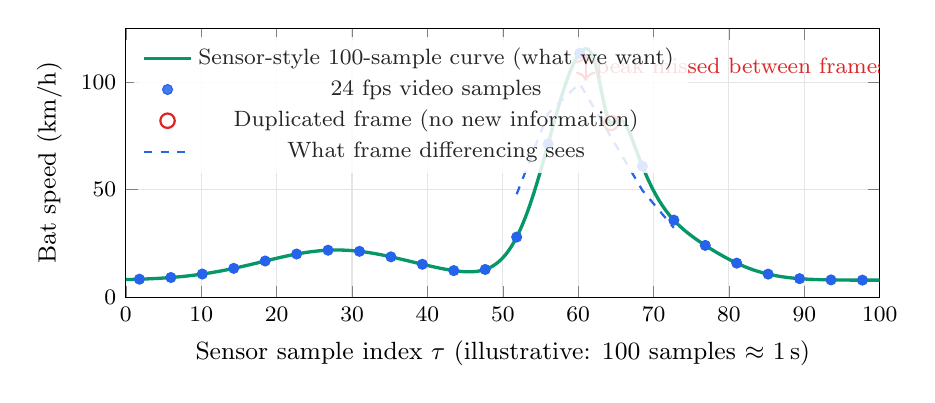
\begin{tikzpicture}
\begin{axis}[
  width=0.92\linewidth, height=5.0cm,
  xmin=0, xmax=100, ymin=0, ymax=125,
  xlabel={Sensor sample index $\tau$ (illustrative: 100 samples $\approx$ 1\,s)},
  ylabel={Bat speed (km/h)},
  ylabel style={font=\small}, xlabel style={font=\small},
  tick label style={font=\footnotesize},
  legend style={font=\footnotesize, at={(0.01,0.97)}, anchor=north west, draw=none, fill=white, fill opacity=0.85},
  grid=major, grid style={gray!20},
]
\addplot[name path=dense, domain=0:100, samples=400, very thick, sen]
  {8 + 14*exp(-((x-28)^2)/(2*10^2)) + 100*exp(-((x-61)^2)/(2*5^2)) - 22*exp(-((x-64)^2)/(2*1.1^2)) + 22*exp(-((x-71)^2)/(2*7^2))};
\addlegendentry{Sensor-style 100-sample curve (what we want)}
\addplot[only marks, mark=*, mark size=1.8pt, vid,
  samples at={1.80,5.97,10.14,14.31,18.48,22.65,26.82,30.99,35.16,39.33,43.50,47.67,51.84,56.01,60.18,68.52,72.69,76.86,81.03,85.20,89.37,93.54,97.71}]
  {8 + 14*exp(-((x-28)^2)/(2*10^2)) + 100*exp(-((x-61)^2)/(2*5^2)) - 22*exp(-((x-64)^2)/(2*1.1^2)) + 22*exp(-((x-71)^2)/(2*7^2))};
\addlegendentry{24 fps video samples}
\addplot[only marks, mark=o, mark size=2.6pt, outc, thick, samples at={64.35}]
  {8 + 14*exp(-((x-28)^2)/(2*10^2)) + 100*exp(-((x-61)^2)/(2*5^2)) - 22*exp(-((x-64)^2)/(2*1.1^2)) + 22*exp(-((x-71)^2)/(2*7^2))};
\addlegendentry{Duplicated frame (no new information)}
\addplot[dashed, vid, thick] coordinates {(51.84,47.9) (56.01,85.4) (60.18,99.4) (68.52,49.7) (72.69,32.3)};
\addlegendentry{What frame differencing sees}
\draw[<->, outc, thick] (axis cs:61,100.5) -- (axis cs:61,113) node[midway, right, font=\footnotesize, text=outc] {peak missed between frames};
\end{axis}
\end{tikzpicture}
\caption{Illustrative (not measured). With $\sim$4 sensor samples per video frame, the true peak and the impact dip fall between frames, and a duplicate frame at impact doubles the gap. Fitting the sensor-learned shape through the video samples recovers the curve between them. Interpolating the samples directly cannot.}
\label{fig:alias}
\end{figure}

\subsection{Build order}
\begin{enumerate}[label=\textbf{\arabic*.}]
  \item \textbf{Baseline (weeks 1--2):} S0 + S1 (stump scale) + S2 pose. Regress a single shape template from the sensor library through the observed wrist speeds. This is already better than raw differentiation, and it is the slice Part~2 proves.
  \item \textbf{Prior + simulator (weeks 3--6):} O1--O4. Train $E_\theta$ on synthetic pairs and test on held-out synthetic swings.
  \item \textbf{Full fusion (weeks 6--10):} PnP calibration, bat and blur heads, ball-exit term, test-time optimisation, uncertainty.
  \item \textbf{Ground truth (in parallel):} a small paired capture session (see Validation). It is the single most valuable dataset for this problem.
\end{enumerate}

\subsection{Hardest risks}\label{sec:risks}
\begin{table}[H]
\centering\small
\renewcommand{\arraystretch}{1.18}
\begin{tabularx}{\linewidth}{>{\raggedright\arraybackslash}p{3.3cm} >{\raggedright\arraybackslash}X >{\raggedright\arraybackslash}X}
\toprule
\textbf{Risk} & \textbf{Why it bites on broadcast footage} & \textbf{Mitigation} \\
\midrule
Depth ambiguity & Down-the-pitch camera: straight drives move along the optical axis. In Part~2 a guessed 50$^\circ$ angle changes speed by 31\%. & Swing-plane azimuth from 3D body lift, footwork and ball exit direction. Shot-conditioned prior. Report the band, not just a point. \\
Temporal aliasing \& pulldown & 4--5 frames per downswing, and 1 in 5 frames can be a duplicate. Finite differences under-read the peak. & S0 removes duplicates. The sensor shape is fitted through the samples instead of interpolating between them. \\
Bat invisible at peak & Blur and occlusion in exactly the frames that matter. & Lever-arm coupling to wrists. Blur direction. Prior fills the gaps and the uncertainty widens there. \\
Sim-to-real gap & The encoder is trained only on simulated tracks. & Corrupt synthetic tracks with noise statistics measured on real clips (Part~2 flags). Test-time optimisation against real evidence. \\
Scale shrinkage & An amateur-heavy library pulls elite speeds down. & Prior on \emph{shape} only. Scale comes from geometry and ball exit. Check per-player bias. \\
Unknown sensor content (A1/A2) & If only scalar speed, or an unknown time base, the alignment weakens. & Settle this first with the data owners. Fall back to a speed-only prior plus impact anchoring. \\
\bottomrule
\end{tabularx}
\end{table}

\subsection{How we would know the estimate is any good}
\begin{enumerate}[label=\textbf{V\arabic*}]
  \item \textbf{Synthetic hold-out:} render held-out sensor swings through the simulator with unseen cameras. Report per-sample RMSE, impact-speed MAE, peak-timing error and 90\%-band coverage. This tests the method, not realism.
  \item \textbf{Paired capture (decisive):} film 200--500 shots by sensor-equipped batters with broadcast-like cameras (behind the bowler, 25--50\,fps, zoom and pan). This is the only true end-to-end test. It also calibrates the uncertainty.
  \item \textbf{Physics checks on real broadcast:} predicted impact speed against ball-exit speed via $e_A$. Wrist-to-sweet-spot ratio within the physical range.
  \item \textbf{Population checks:} for each shot type, the predicted distribution across many broadcast shots should sit plausibly against the sensor distribution. The same batter's repeated shots should be consistent, and harder shots should rank higher.
\end{enumerate}
\textbf{Target (assumption):} impact speed within $\pm$8\,km/h, peak timing within $\pm$1 frame, and 90\% bands that contain the truth about 90\% of the time.

% ==================================================================
\newpage
\section{Part 2: A working slice on real broadcast footage}
% ==================================================================
\subsection{Clip and setup}
\begin{minipage}[t]{0.66\linewidth}
\vspace{0pt}
A public broadcast clip of Liam Livingstone (England v Pakistan T20, main camera behind the bowler) playing a lofted on-side drive:
720$\times$1280 portrait, 29.95\,fps, 72 frames (2.40\,s). Frames 0--21 are a different camera shot before a cut. The batting shot is frames 22--71.
This slice implements S0, S1 (stump-scale fallback) and S2 (pose) from Figure~\ref{fig:arch}, plus a lever-arm bat proxy.

\begin{enumerate}
  \item \textbf{S0:} frame extraction, cut detection, duplicate detection (mean absolute grey difference $<1.5$).
  \item \textbf{S1:} Lucas--Kanade flow on background features with YOLOv8 people masks, partial-affine RANSAC for camera $\Delta x,\Delta y$, and stump-height scale.
  \item \textbf{S2:} YOLOv8x-pose (COCO-17) in a striker corridor ROI. Wrist gating and imputation. Camera-motion subtraction. PCHIP interpolation over unique frames only. Savitzky--Golay derivatives.
  \item \textbf{Bat proxy:} blade direction from the forearm vector refined by an image-gradient search (not a bat detector), then $\vec v_{\text{bat}}=\vec v_{\text{pivot}}+\omega r\,\hat n_\perp$ with $r=0.55$\,m.
\end{enumerate}
Code: \texttt{run\_pipeline.py}, \texttt{src/camera\_motion.py}, \texttt{src/track\_swing.py}, \texttt{src/plot\_velocity.py}.
\end{minipage}\hfill
\begin{minipage}[t]{0.31\linewidth}
\vspace{0pt}
\centering
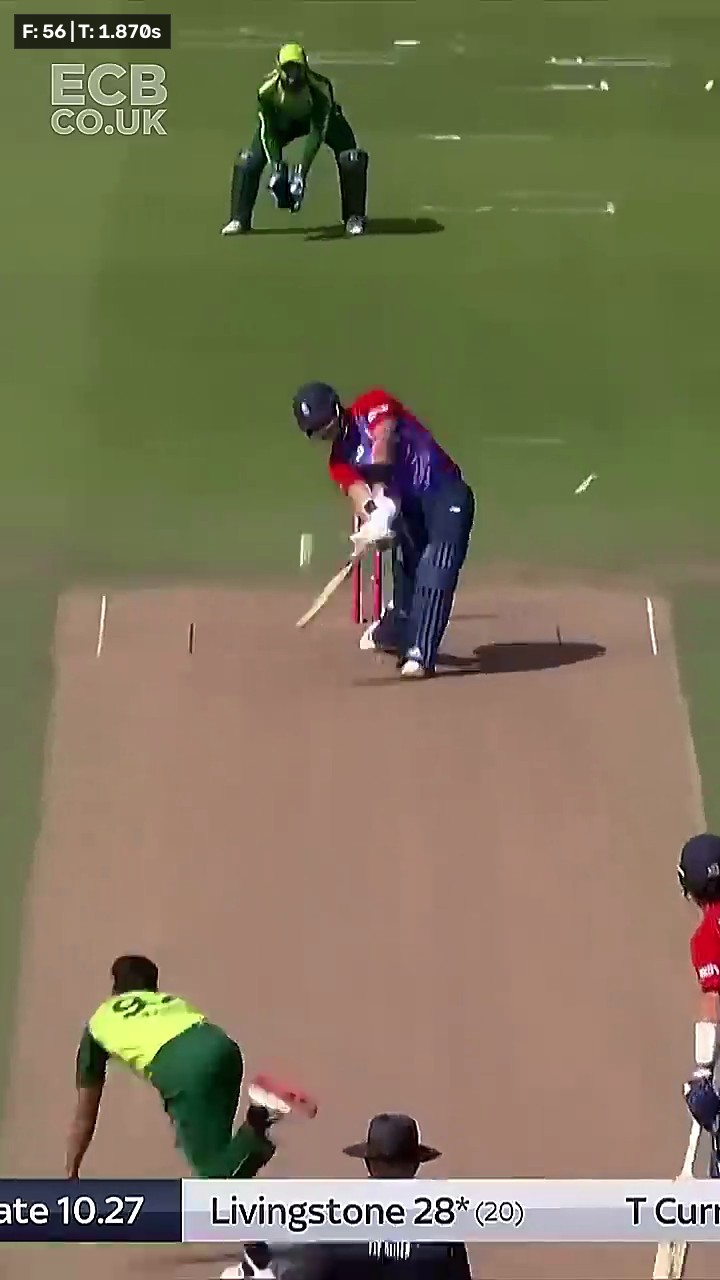
\includegraphics[width=\linewidth,trim=0 380 0 0,clip]{figures/frame56_full.jpg}
\captionof{figure}{Frame 56 (top of frame). The batter is about 150\,px tall, and the stumps used for scale are 99\,px.}
\label{fig:frame}
\end{minipage}

\begin{table}[H]
\centering\small
\caption{Calibration and clip facts.}
\label{tab:calib}
\begin{tabular}{@{}lll@{}}
\toprule
\textbf{Quantity} & \textbf{Value} & \textbf{How obtained} \\
\midrule
Resolution / frame rate & 720$\times$1280 / 29.954 fps & container ($\Delta t = 33.4$\,ms) \\
Frames / duration & 72 / 2.404 s & shot window: frames 22--71 (50 frames) \\
Duplicate frames & 14 in clip, 10 in shot & every 5th frame: 23, 27, 32, \dots, 57, 62, 67 \\
Effective source rate & $\approx$24 fps & 1 duplicate per 5 frames $\Rightarrow$ 2:3 pulldown \\
Stump height in image & 99.25 px & top (340, 809), base (333, 908) \\
Scale at crease plane & 0.007164 m/px (7.16 mm/px) & 0.711 m / 99.25 px \\
px/s $\to$ km/h & $\times\,0.02579$ & $0.007164 \times 3.6$ \\
Camera speed in shot & mean 15.7, max 140.3 px/s & frames 29--31, delivery pan \\
\bottomrule
\end{tabular}
\end{table}

\subsection{Velocity profile across the swing}
Figure~\ref{fig:vel} is the main result. It is plotted directly from \texttt{swing\_kinematics.csv}. The raw (grey) curve is the naive frame-to-frame handle speed. The green curve is after duplicate removal, camera compensation and wrist gating. The red and purple curves are the bat-proxy sweet spot in 2D and with the out-of-plane correction.

\begin{figure}[H]
\centering
\begin{tikzpicture}
\begin{axis}[
  name=main,
  width=0.94\linewidth, height=7.0cm,
  xmin=22, xmax=71, ymin=0, ymax=82,
  ylabel={Speed (km/h)}, xlabel={},
  xtick={22,25,...,70}, xticklabels={},
  tick label style={font=\footnotesize},
  ylabel style={font=\small},
  grid=major, grid style={gray!18},
  legend style={font=\scriptsize, at={(0.01,0.97)}, anchor=north west, draw=gray!40, fill=white, fill opacity=0.9, text opacity=1, row sep=-1pt},
  legend cell align=left,
  clip=false,
]
% phase bands
\fill[cStance] (axis cs:22,0) rectangle (axis cs:47.5,82);
\fill[cBack]   (axis cs:47.5,0) rectangle (axis cs:54.5,82);
\fill[cDown]   (axis cs:54.5,0) rectangle (axis cs:56.5,82);
\fill[cImp]    (axis cs:56.5,0) rectangle (axis cs:57.5,82);
\fill[cFT]     (axis cs:57.5,0) rectangle (axis cs:71,82);
\node[font=\scriptsize\bfseries, text=orange!70!black, anchor=south] at (axis cs:34.75,82.5) {STANCE (22--47)};
\node[font=\scriptsize\bfseries, text=vid, anchor=south] at (axis cs:51,82.5) {BACKLIFT};
\node[font=\scriptsize\bfseries, text=orange!80!black, rotate=90, anchor=west] at (axis cs:55.5,83) {DOWN};
\node[font=\scriptsize\bfseries, text=outc, rotate=90, anchor=west] at (axis cs:57,83) {IMPACT};
\node[font=\scriptsize\bfseries, text=fus, anchor=south] at (axis cs:65.3,82.5) {FOLLOW-THROUGH (58--71)};
% duplicate frame markers
\foreach \d in {23,27,32,37,42,47,52,57,62,67} {
  \edef\tmp{\noexpand\draw[gray!70, densely dotted, line width=0.6pt] (axis cs:\d,0) -- (axis cs:\d,82);}
  \tmp
}
\addplot[gray!70, line width=0.8pt, mark=none] table[x=frame,y=rawpiv]{figures/kin.dat};
\addlegendentry{Raw handle pivot}
\addplot[teal, line width=1.6pt] table[x=frame,y=piv]{figures/kin.dat};
\addlegendentry{Handle pivot, stabilised + de-duplicated}
\addplot[outc, line width=1.6pt] table[x=frame,y=bat2d]{figures/kin.dat};
\addlegendentry{Bat proxy, 2D projected}
\addplot[fus, line width=1.4pt, dashed] table[x=frame,y=bat3d]{figures/kin.dat};
\addlegendentry{Bat proxy, $1/\sin\phi$ (assumed $\phi$)}
\addlegendimage{gray!70, densely dotted, line width=0.6pt}
\addlegendentry{Duplicate (pulldown) frame}
% annotations
\node[circle, fill=fus, inner sep=1.4pt] at (axis cs:56,74.87) {};
\node[font=\scriptsize, text=fus, anchor=east, fill=white, fill opacity=0.8, text opacity=1, inner sep=1pt] (l3) at (axis cs:53.6,74) {74.9 km/h (3D est.)};
\draw[fus, thin] (l3.east) -- (axis cs:55.8,74.8);
\node[circle, fill=outc, inner sep=1.4pt] at (axis cs:56,57.36) {};
\node[font=\scriptsize, text=outc, anchor=west, fill=white, fill opacity=0.8, text opacity=1, inner sep=1pt] (l2) at (axis cs:61.5,70) {57.4 km/h (2D)};
\draw[outc, thin] (l2.west) -- (axis cs:56.2,57.6);
\node[circle, fill=teal, inner sep=1.4pt] at (axis cs:56,33.84) {};
\node[font=\scriptsize, text=teal, anchor=west, fill=white, fill opacity=0.8, text opacity=1, inner sep=1pt] (l1) at (axis cs:63,40) {33.8 km/h handle};
\draw[teal, thin] (l1.west) -- (axis cs:56.2,33.9);
\node[font=\scriptsize, text=gray!50!black, anchor=west, align=left, fill=white, fill opacity=0.8, text opacity=1, inner sep=1pt] (l0) at (axis cs:63,27) {F57 raw: 0.9 km/h\\(duplicate frame)};
\draw[gray!50!black, thin, ->] (l0.west) -- (axis cs:57.15,1.3);
\end{axis}

% ---- inter-wrist distance + trail-wrist confidence
\begin{axis}[
  name=wr,
  at={(main.below south west)}, anchor=above north west, yshift=-0.25cm,
  width=0.94\linewidth, height=3.4cm,
  xmin=22, xmax=71, ymin=0, ymax=110,
  ylabel={Wrist gap (px)}, ylabel style={font=\small, text=fus},
  xtick={22,25,...,70}, xticklabels={},
  tick label style={font=\footnotesize},
  grid=major, grid style={gray!18},
  axis y line*=left,
]
\fill[green!12] (axis cs:22,10) rectangle (axis cs:71,45);
\node[font=\scriptsize, text=green!40!black, anchor=west] at (axis cs:22.3,30) {grip band 10--45 px};
\addplot[fus, line width=1.1pt, mark=*, mark size=0.9pt] table[x=frame,y=wd]{figures/kin.dat};
\end{axis}
\begin{axis}[
  at={(wr.south west)}, anchor=south west,
  width=0.94\linewidth, height=3.4cm,
  xmin=22, xmax=71, ymin=0, ymax=1.1,
  ylabel={Trail-wrist conf.}, ylabel style={font=\small, text=orange!80!black},
  axis y line*=right, axis x line=none,
  tick label style={font=\footnotesize},
]
\addplot[orange!85!black, line width=1.0pt, densely dashed] table[x=frame,y=rwc]{figures/kin.dat};
\addplot[gray, thin, dashed, domain=22:71] {0.55};
\end{axis}

% ---- camera speed
\begin{axis}[
  name=cam,
  at={(wr.below south west)}, anchor=above north west, yshift=-0.25cm,
  width=0.94\linewidth, height=2.9cm,
  xmin=22, xmax=71, ymin=0, ymax=160,
  ylabel={Camera (px/s)}, ylabel style={font=\small},
  xtick={22,25,...,70}, xticklabels={},
  tick label style={font=\footnotesize},
  grid=major, grid style={gray!18},
]
\addplot[ink, line width=1.0pt, fill=gray!25] table[x=frame,y=cam]{figures/kin.dat} \closedcycle;
\addplot[outc, dashed, thin, domain=22:71] {120};
\node[font=\scriptsize, text=outc, anchor=west] at (axis cs:40,70) {dashed: pan threshold 120 px/s};
\end{axis}

% ---- failure flag ribbon
\begin{axis}[
  at={(cam.below south west)}, anchor=above north west, yshift=-0.2cm,
  width=0.94\linewidth, height=1.7cm,
  xmin=22, xmax=71, ymin=0, ymax=1,
  ytick=\empty, ylabel={Flag}, ylabel style={font=\small},
  xtick={22,25,...,70}, xlabel={Video frame}, xlabel style={font=\small},
  tick label style={font=\footnotesize},
  clip=true,
]
\foreach \a/\b/\c in {22/28/fOCC,29/31/fCAM,32/53/fOCC,54/56/fOK,57/57/fBLUR,58/58/fOK,59/59/fOCC,60/60/fOK,61/62/fOCC,63/67/fOK,68/68/fOCC,69/71/fOK} {
  \edef\tmp{\noexpand\fill[\c] (axis cs:\a-0.5,0.1) rectangle (axis cs:\b+0.5,0.9);}
  \tmp
}
\end{axis}
\end{tikzpicture}

\vspace{2pt}
{\footnotesize
\tikz\fill[fOK] (0,0) rectangle (0.3,0.2); OK \quad
\tikz\fill[fOCC] (0,0) rectangle (0.3,0.2); OCCLUSION \quad
\tikz\fill[fCAM] (0,0) rectangle (0.3,0.2); CAMERA\_EGO\_MOTION \quad
\tikz\fill[fBLUR] (0,0) rectangle (0.3,0.2); MOTION\_BLUR\_DROPOUT}
\caption{Velocity profile across the swing (frames 22--71), plotted from \texttt{swing\_kinematics.csv}. \textbf{Top:} speed in km/h (px/s $= $ km/h $/\,0.02579$). Dotted verticals mark duplicate frames. \textbf{Second:} inter-wrist distance (purple, left axis) against the plausible grip band, and trail-wrist confidence (orange dashed, right axis; grey line is the 0.55 gating threshold). \textbf{Third:} background camera speed. \textbf{Bottom:} per-frame tracking flag.}
\label{fig:vel}
\end{figure}

\begin{table}[H]
\centering\small
\caption{Kinematic results (shot window, frames 22--71).}
\label{tab:kin}
\begin{tabular}{@{}lrrl@{}}
\toprule
\textbf{Metric} & \textbf{px/s} & \textbf{km/h} & \textbf{Frame / note} \\
\midrule
Peak handle-pivot speed (stabilised) & 1312 & 33.8 & F56, late downswing \\
Peak bat sweet-spot proxy, 2D projected & 2224 & 57.4 & F56 \\
Peak bat proxy, $1/\sin 50^\circ$ corrected & 2903 & 74.9 & F56; $\phi$ assumed, not measured \\
Bat-to-handle ratio at peak & \multicolumn{2}{c}{1.70$\times$} & lever-arm contribution $\approx$ +23.5 km/h \\
Bat proxy at impact window & 2031 & 52.4 (68.4 corr.) & F57 is a duplicate of F56 \\
Raw pivot speed at F57 & 34 & 0.9 & artefact of duplicate frame \\
Raw pivot peak (uncorrected) & 2003 & 51.7 & F54: wrist label jump, not motion \\
\bottomrule
\end{tabular}
\end{table}

\subsection{What it takes to get real-world units}
The km/h axis above uses one scale factor: the stump height at the crease plane. That is a first-order conversion. A trustworthy one needs four more things:
\begin{enumerate}
  \item \textbf{Depth-correct scale.} The batter stands about 1.2\,m in front of the stumps, closer to the camera, so 7.16\,mm/px is slightly wrong for the hands. A full PnP from crease corners plus the vertical stump gives scale at the batter's actual depth.
  \item \textbf{The out-of-plane component.} A down-the-pitch camera cannot see motion along its axis. I applied $1/\sin\phi$ with $\phi = 50^\circ$ in the downswing, which adds 31\%. That angle is a modelling assumption. It should come from the swing plane (3D body lift and ball direction), or better, from the sensor prior.
  \item \textbf{Sub-frame timing.} At an effective 24\,fps with the impact frame duplicated, frames 56 to 58 span 67\,ms. The real peak is sharper than any finite difference can show (Figure~\ref{fig:alias}).
  \item \textbf{Actual bat tracking.} The sweet-spot speed comes from a forearm-direction proxy and an assumed 0.55\,m lever. A bat keypoint or blur model would replace the assumption with a measurement.
\end{enumerate}
The 74.9\,km/h estimate is well below the 100\,km/h-plus typical of an elite power hit. I read that gap as a measure of what these four corrections are still missing, not as a finding about the batter.

\subsection{Where tracking failed, and why}
Of the 50 shot frames, 13 (26\%) tracked cleanly. Figure~\ref{fig:strip} shows each failure type and Table~\ref{tab:fail} counts them.

\begin{figure}[H]
\centering
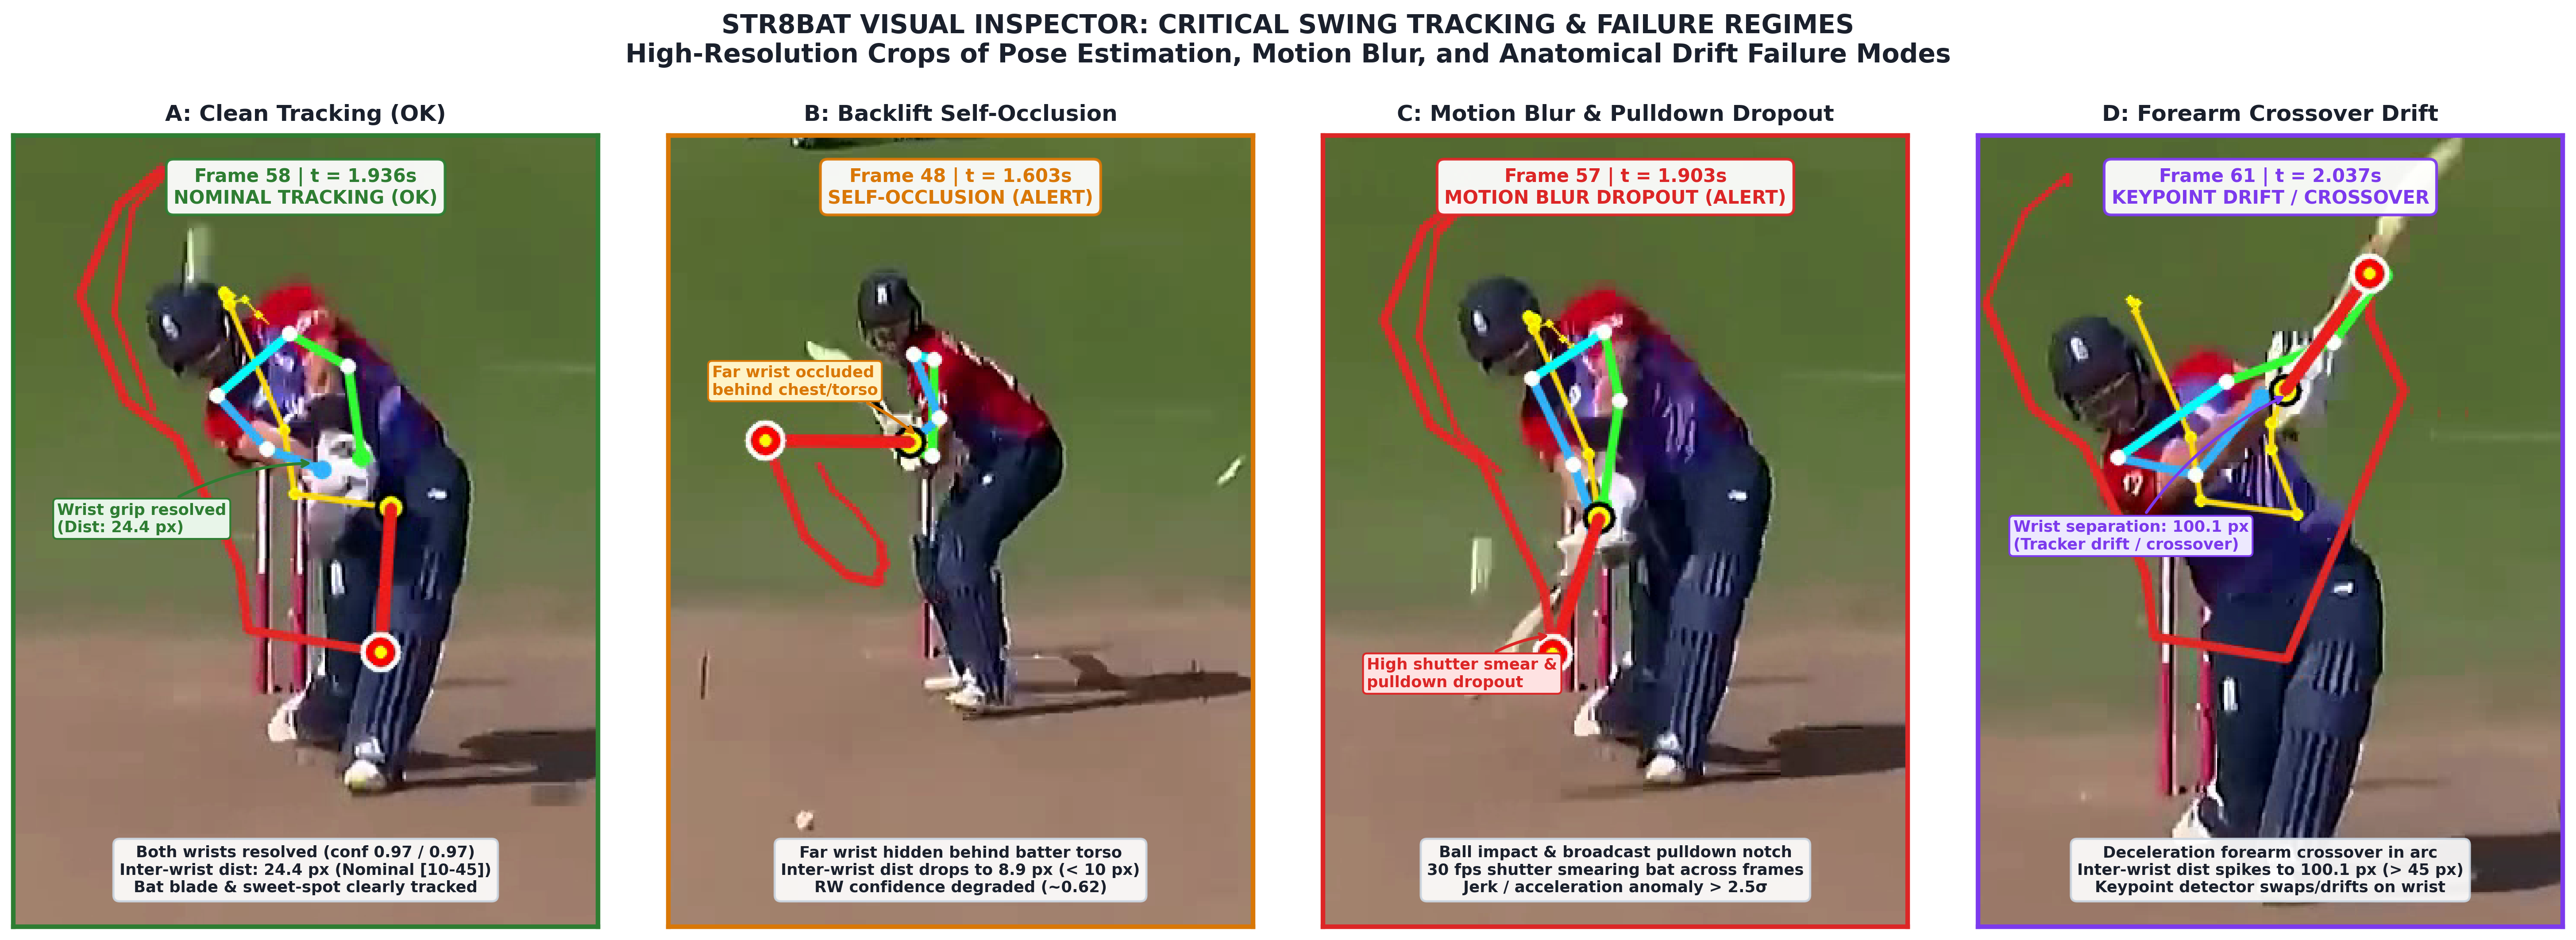
\includegraphics[width=\linewidth]{figures/failure_frames_strip.png}
\caption{Pipeline output on four representative frames. \textbf{A} (F58): clean two-wrist tracking. \textbf{B} (F48): trail wrist hidden behind the torso. \textbf{C} (F57): impact frame, which is a pulldown duplicate with blade smear. \textbf{D} (F61): forearm crossover in follow-through. Wrist labels drift and the separation jumps to 100\,px.}
\label{fig:strip}
\end{figure}

\begin{figure}[H]
\centering
\begin{subfigure}{0.24\linewidth}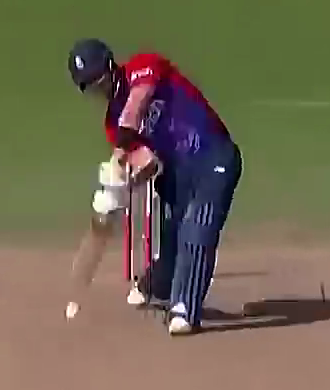
\includegraphics[width=\linewidth]{figures/crop_55.png}\caption*{F55, $t$=1.836 s}\end{subfigure}\hfill
\begin{subfigure}{0.24\linewidth}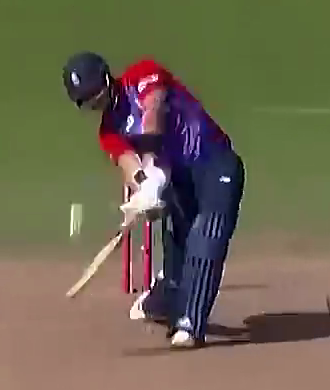
\includegraphics[width=\linewidth]{figures/crop_56.png}\caption*{F56, $t$=1.870 s}\end{subfigure}\hfill
\begin{subfigure}{0.24\linewidth}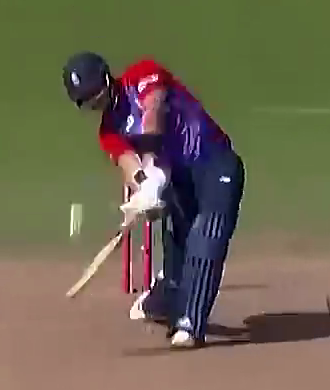
\includegraphics[width=\linewidth]{figures/crop_57.png}\caption*{F57, $t$=1.903 s (= F56)}\end{subfigure}\hfill
\begin{subfigure}{0.24\linewidth}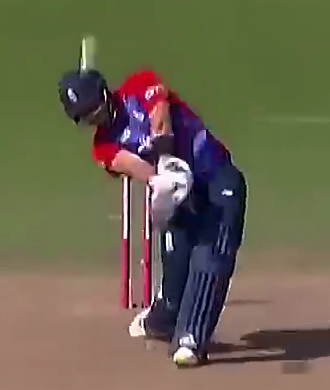
\includegraphics[width=\linewidth]{figures/crop_58.png}\caption*{F58, $t$=1.936 s}\end{subfigure}
\caption{The impact window, uncropped in time. F57 is pixel-identical to F56 (mean absolute difference 0.15 grey levels), so ball--bat contact is never seen. It happens somewhere in the 67\,ms between F56 and F58. Note also how small the bat is at this resolution.}
\label{fig:impact}
\end{figure}

\begin{table}[H]
\centering\small
\caption{Failure flags across the shot window (50 frames), from \texttt{swing\_kinematics.csv}.}
\label{tab:fail}
\renewcommand{\arraystretch}{1.15}
\begin{tabularx}{\linewidth}{@{}>{\raggedright\arraybackslash}p{3.4cm} c c >{\raggedright\arraybackslash}p{2.6cm} >{\raggedright\arraybackslash}X@{}}
\toprule
\textbf{Flag} & \textbf{Frames} & \textbf{\%} & \textbf{Where} & \textbf{Why it broke} \\
\midrule
\textcolor{fOCC}{\textbf{OCCLUSION}} & 33 & 66 & 22--28, 32--53, 59, 61--62, 68 & \emph{Stance/backlift:} the trail wrist is behind the lead forearm and chest. Confidence 0.35--0.65. The model puts both wrists on the visible hand (gap $<$10\,px), or the trail wrist jumps to the elbow or bat top (90\,px at F50). \emph{Follow-through:} the forearms cross, the labels swap or drift onto shoulder or helmet, and the gap reaches 100\,px at F61. \\
\textcolor{fCAM}{\textbf{CAMERA\_EGO\_\allowbreak MOTION}} & 3 & 6 & 29--31 & The camera pans with the bowler's delivery at 130--140 px/s. Without background-flow subtraction this would add phantom batter speed. \\
\textcolor{fBLUR}{\textbf{MOTION\_BLUR\_\allowbreak DROPOUT}} & 1 & 2 & 57 & Impact frame is a pulldown duplicate, and the blade is smeared. Raw pivot speed drops from 31.6 to 0.9\,km/h. \\
\textcolor{fOK}{\textbf{OK}} & 13 & 26 & 54--56, 58, 60, 63--67, 69--71 & Both wrists detected with confidence above 0.85 and no implausible jump in wrist position. \\
\bottomrule
\end{tabularx}
\end{table}

\subsection{What did not work (honest note)}
\begin{itemize}
  \item \textbf{The bat itself was never detected.} The ``bat speed'' is a physics proxy: wrist motion, forearm direction and an assumed lever. At about 150\,px batter height the blade is a few pixels wide and blurred, and off-the-shelf detectors do not find it.
  \item \textbf{Most frames are not clean.} 74\% of shot frames were flagged. The trail wrist is imputed from the lead wrist for most of the stance, so stance-phase speeds rest on one wrist.
  \item \textbf{The peak sits in the worst part of the clip.} The downswing has 3 unique frames, and the impact frame is a duplicate. The smoothed peak depends on the spline and Savitzky--Golay window choices. With a 5-frame window across a 3-frame event, it is a lower bound, not a measurement.
  \item \textbf{The 3D correction is a guess.} $\phi=50^\circ$ is a judgement from watching the shot, so the 74.9\,km/h figure carries that assumption.
  \item \textbf{Gating can hide real motion.} The rules that reject wrist spikes (gap $>$45\,px, confidence $<$0.55) were tuned by eye on this clip and need validation on others.
  \item \textbf{What worked:} duplicate detection, which explained the impact-frame dropout. Camera-motion subtraction during the delivery pan. A failure classifier whose flags match what is visibly wrong in the frames. These map directly onto S0--S2 of the design and onto the noise model the simulator (O3) needs.
\end{itemize}

\subsection{Reproducing}
{\small
\texttt{pip install -r requirements.txt}\\
\texttt{python run\_pipeline.py}\hfill(about 50\,s on a laptop)\\[2pt]
\raggedright Outputs in \texttt{outputs/}: \texttt{swing\_kinematics.csv} (72 rows $\times$ 32 columns), \texttt{camera\_metrics.json}, \texttt{annotated\_swing.mp4}, \texttt{velocity\_profile\_analysis.png}, \texttt{failure\_frames\_strip.png}.\par}

% ==================================================================
\appendix
\section{Appendix: original diagnostic figure}
\begin{figure}[H]
\centering
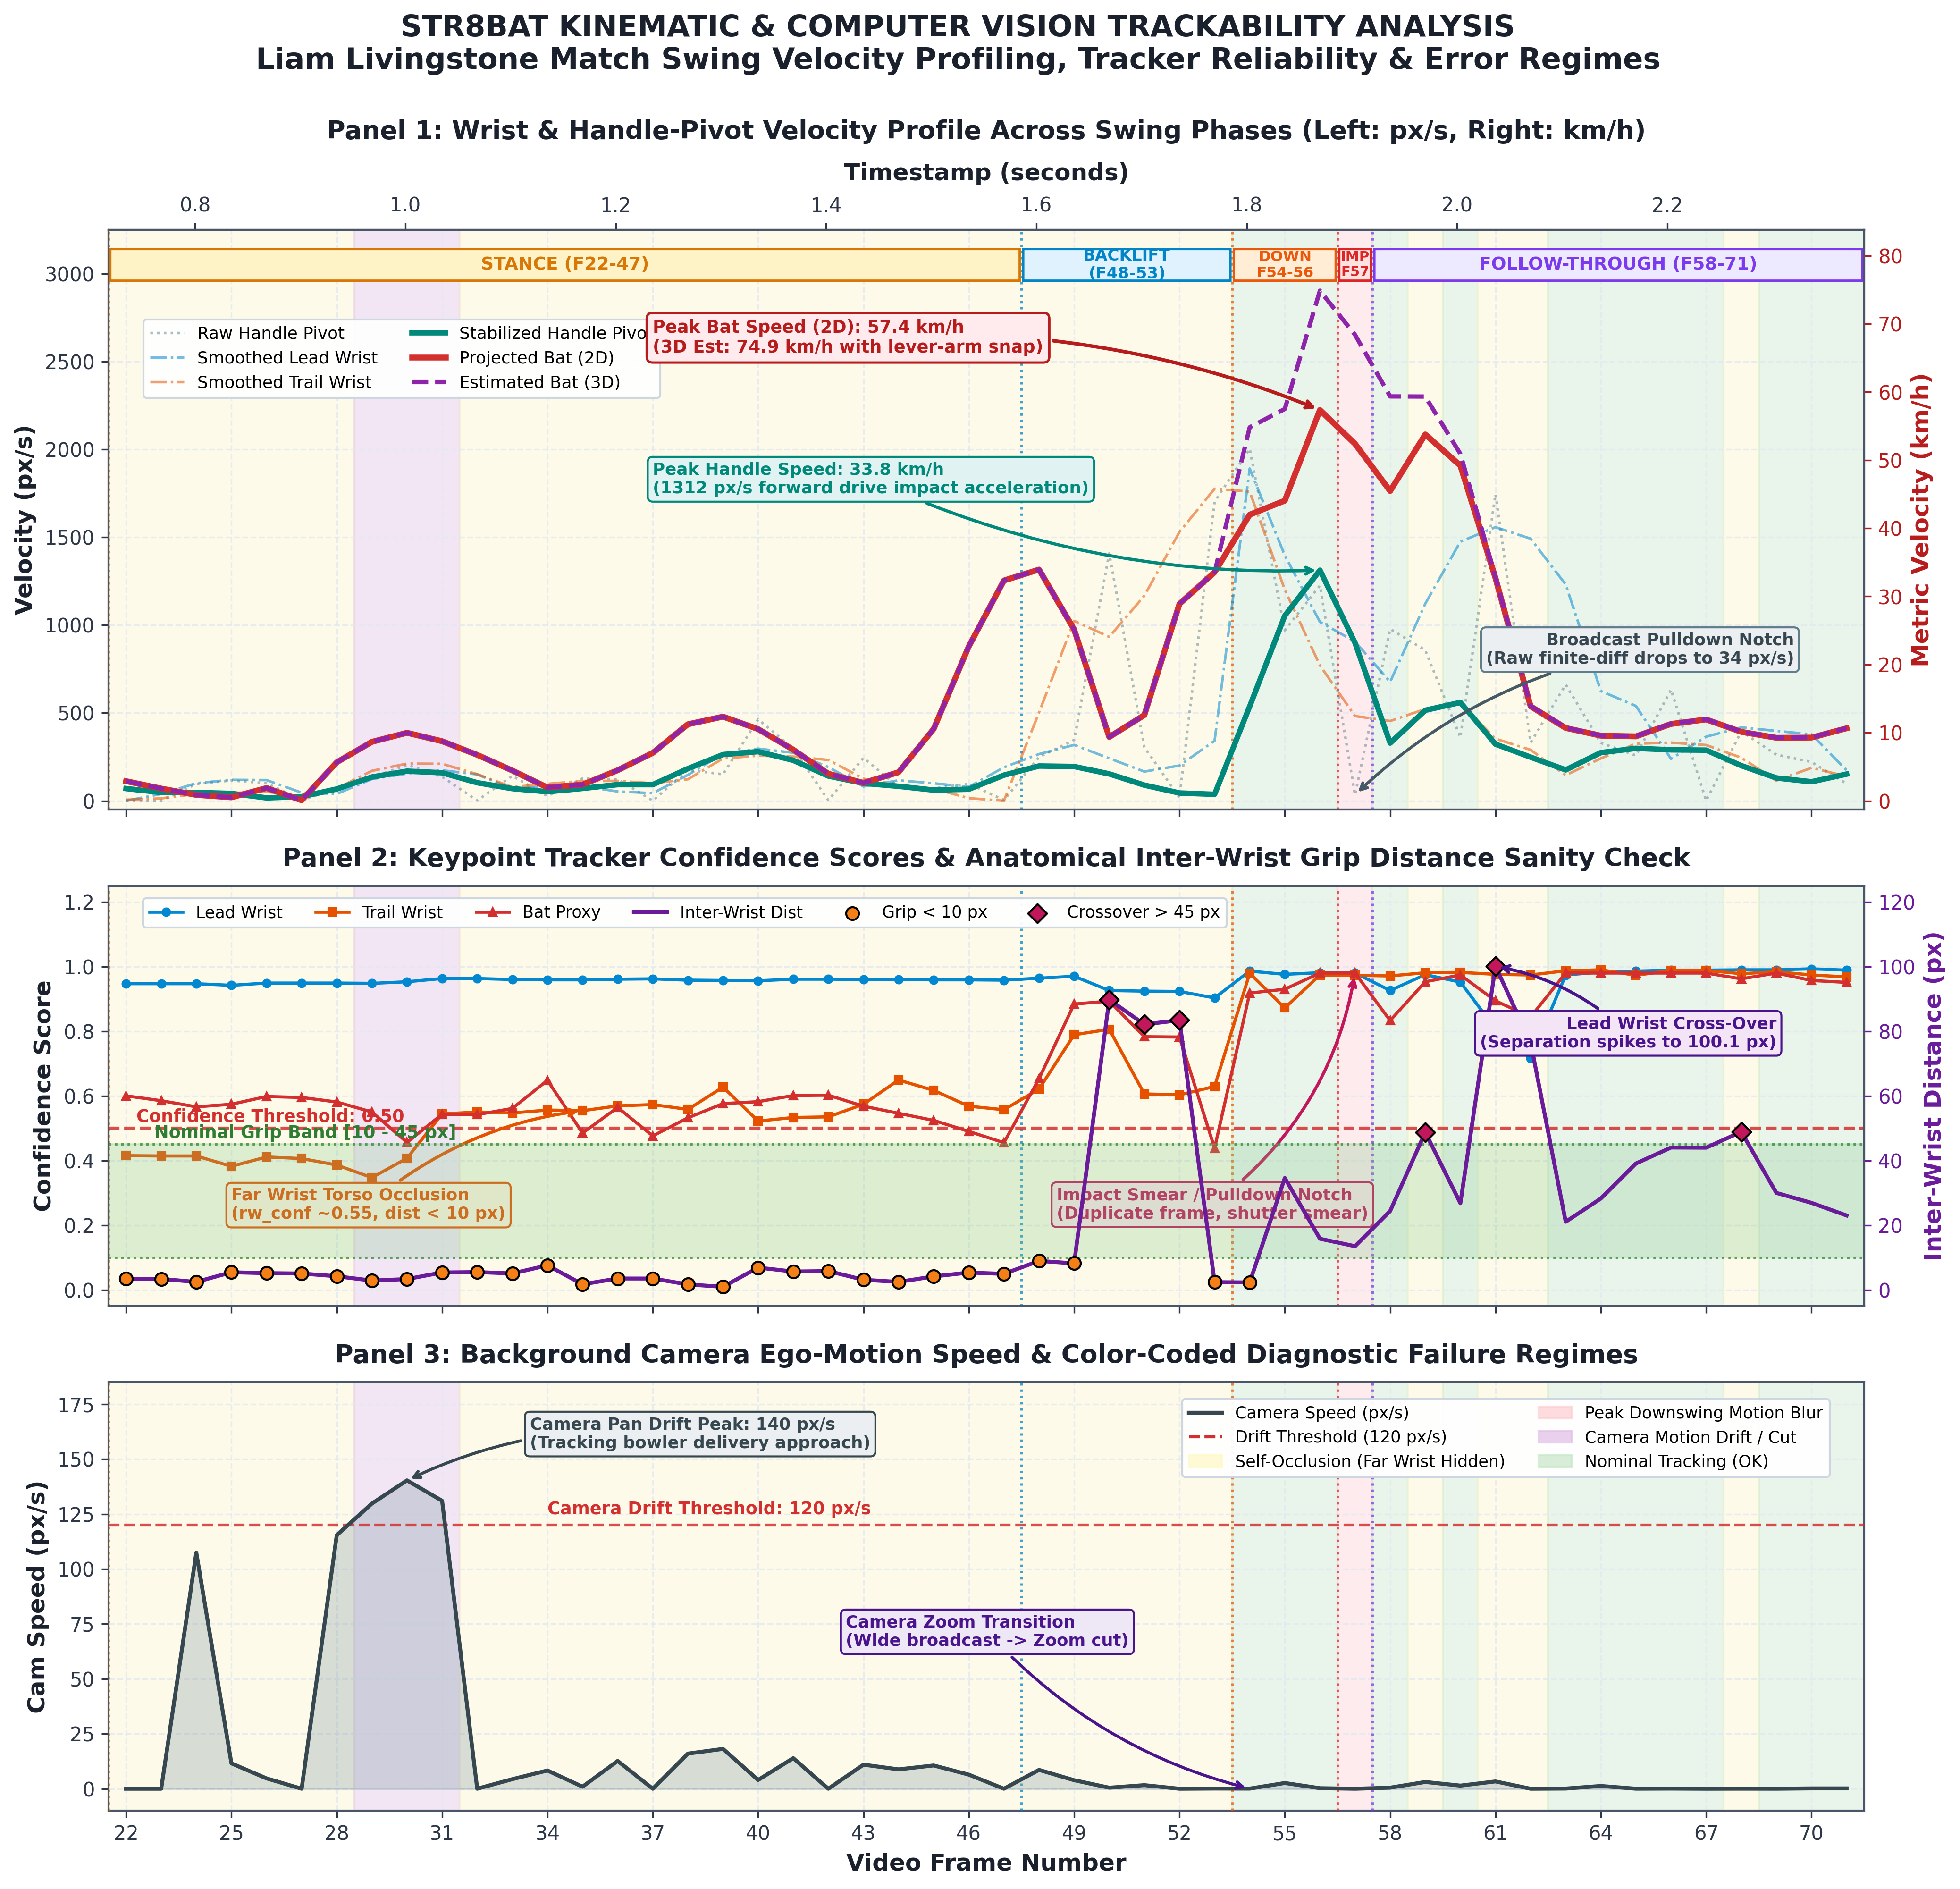
\includegraphics[width=0.94\linewidth]{figures/velocity_profile_analysis.png}
\caption{The pipeline's own 3-panel diagnostic figure (\texttt{outputs/velocity\_profile\_analysis.png}), kept for reference. Figure~\ref{fig:vel} redraws the same data.}
\end{figure}

\end{document}
